\documentclass{standalone}
\usepackage{chez}

\begin{document}
\chapter{September 23, 2020}
Recall \cref{thm:excision}, namely that if \(U \subseteq A \subseteq X\)
with \(\ol U \subseteq \Int(A)\), then the inclusion
\((X - U, A - U) \subseteq (X, A)\) is called an excision.
Then, the last~\hyperref[thm:eilenberg-steenrod]{Eilenberg-Steenrod} axiom
states that excisions induces homology equivalence, i.e.
\(H_m(X - U, A - U) \iso H_m(X, A)\).

The key to excision will be the ``locality principle''.
\begin{definition}
  Let \(X\) be a topological space. A family \(\mathcal A\) of subsets of \(X\)
  is a \vocab{cover} if \(X\) is the union of the interiors of
  \(A \in \mathcal A\).
\end{definition}
\begin{definition}
  If \(\mathcal A\) is a cover of \(X\), an \(n\)-simplex
  \(\sigma \colon \Delta^n \to X\) is \vocab{\(\mathcal A\)-small}
  if the image of \(\sigma\) is entirely contained in
  a single element of \(\mathcal A\).
\end{definition}

Note that if \(\sigma \colon \Delta^n \to X\) is \(\mathcal A\)-small,
then so is \(d_i \sigma\) for \(0 \leq i \leq n\).
This means that we can form a semisimplicial set
\(\Sing^{\mathcal A}(X)\) with \(n\)-simplices that are
the \(\mathcal A\)-small \(n\)-simplices in \(X\).
Furthermore, a chain complex \(S_*^{\mathcal A}(X)\) can be formed.

\begin{theorem}[Locality principle]<locality>
  The inclusion \(S_*^{\mathcal A}(X) \subseteq S_*(X)\)
  induces isomorphisms on homology groups.
\end{theorem}

To show this, we want to show that a cycle in \(Z_n(X)\) is equivalent
to a cycle that is the sum of smaller simplices, i.e\ is \(\mathcal A\)-small.
We can do this by adding boundaries.

\begin{figure}
  \centering
  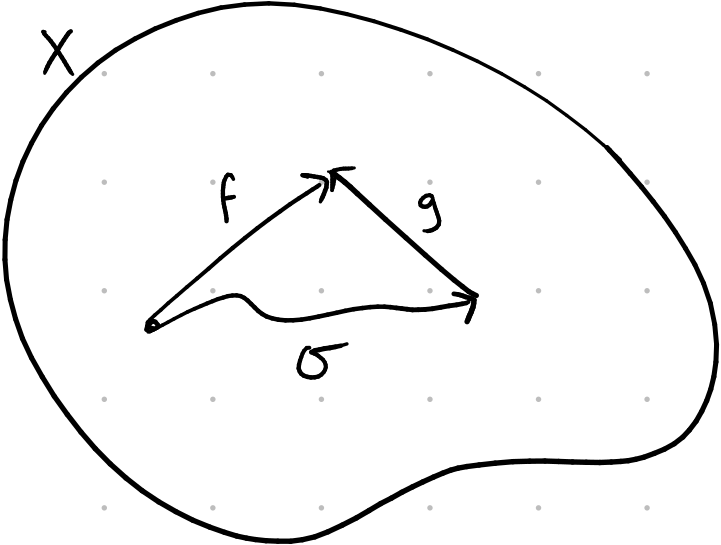
\includegraphics[width=0.25\textwidth]{18_905-200923-1.png}
  \caption{a \(1\)-simplex in \(X\)}%
  \label{fig:locality-1}
\end{figure}
For intuition, if we have some \(\sigma \colon \Delta^1 \to X\),
we can consider two other simplices \(f, g\) such that \(f - g - \sigma = 0\)
in \(H_1(X)\), as shown in \cref{fig:locality-1}.
If we let the endpoints of \(f\) and \(g\) be the midpoint of \(\sigma\),
then we will have \(\sigma = f - g\), modulo \(\partial\).
If we repeat this process, we will eventually have simplices that are
\(\mathcal A\)-small.

To make this precise, we will construct a natural transformation
\[
  \$ \colon S_n \to S_n.
\]
In other words, for any \(X \in \cAb\), we will construct a map
\(\$ \colon S_n(X) \to S_n(X)\). To do so, we need to say what it does
to a generator \(\sigma \colon \Delta^n \to X\).

Consider the naturality square
\[
  \begin{tikzcd}
    S_n(\Delta^n) \arrow[r, "\$"] \arrow[d, "S_n(\sigma)"'] &
      S_n(\Delta^n) \arrow[d, "S_n(\sigma)"] \\
    S_n(X) \arrow[r, "\$"'] &
      S_n(X)
  \end{tikzcd}
\]
which commutes if \(\$\) is natural. There is a special \(n\)-simplex
\[
  1_{\Delta^n} \colon \Delta^n \to \Delta^n.
\]
\(1_{\Delta^n} \in S_n(\Delta^n)\) is one of the generators of the
free abelian group.
Note that \(S_n(\sigma)(1_{\Delta^n}) = \sigma \in S_n(X)\).
Naturality says
\[
  \$(\sigma) = S_n(\sigma)(\$(1_{\Delta^n})).
\]
Therefore, if we specify \(\$(1_{\Delta^n})\), then we specify \(\$\).

\begin{figure}
  \centering
  \begin{subfigure}[b]{0.4\textwidth}
    \centering
    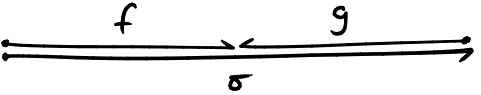
\includegraphics[width=0.7\textwidth]{18_905-200923-2.png}
    \caption{\(\$(1_{\Delta^1})\)}
  \end{subfigure}
  \begin{subfigure}[b]{0.4\textwidth}
    \centering
    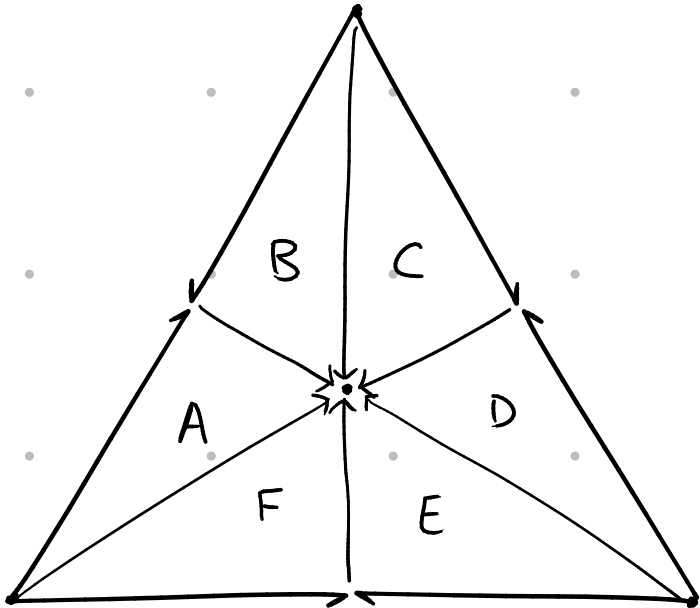
\includegraphics[width=0.7\textwidth]{18_905-200923-3.png}
    \caption{\(\$(1_{\Delta^2})\)}
  \end{subfigure}
  \caption{Diagrams specifying \(\$\)}%
  \label{fig:locality-2}
\end{figure}
\begin{itemize}[nosep]
  \item For \(\Delta^0\), we define \(\$(1_{\Delta^0}) = 1_{\Delta^0}\),
    meaning that if we have \(\Delta^0\), meaning that we do not need to subdivide a point to make it more local.
  \item For \(\Delta^1\), we let \(\$(1_{\Delta^1}) = f - g \in S_1(\Delta^1)\),
    as given by \cref{fig:locality-2}.
  \item For \(\Delta^2\), we let
    \(\$(1_{\Delta^2}) = A-B+C-D+E-F \in S_1(\Delta^2)\),
    also as given by \cref{fig:locality-2}.
\end{itemize}
If we calculate the boundary of these expressions, we get the same thing as
what we would have if we took the boundary of \(\Delta^1\) or \(\Delta^2\).
We think of these expressions as equivalent under homology, but more local.

More generally, to define \(\$(1_{\Delta^n})\), we let \(b\) denote the
center of mass of \(\Delta^n\). We subdivide the boundary of \(\Delta^n\)
according to \(\$\) in one lower dimension, and then connect everything
to \(b\). In particular,
\[
  \$ 1_{\Delta^n} = b \ast \$(\partial 1_{\Delta^n}),
\]
where \(b \ast {-} \colon S_{n-1}(\Delta^n) \to S_n(\Delta^n)\) is the cone
construction for star shaped regions defined for star-shaped regions.

\begin{theorem}
  For any topological space \(X\),
  \[
    \$ \colon S_*(X) \to S_*(X)
  \]
  is a chain map. Furthermore, it is chain homotopic to the identity.
\end{theorem}

\begin{proof}
  Note that we have \(\partial \$ 1_{\Delta^n} = \$ \partial 1_{\Delta^n}\)
  from the definition of the construction of \(\$\).
  It follows by naturailty of \(\$\) that if \(\sigma \colon \Delta^n \to X\)
  is any \(n\)-simplex,
  \[
    \partial \$ \sigma = \partial \$(S_n(\sigma)(1_{\Delta^n}))
      = S_n(\sigma)(\partial \$ 1_{\Delta^n})
      = S_n(\sigma)(\$\partial 1_{\Delta^n})
      = \$ \partial \sigma.
  \]
  Therefore, \(\$\) is a chain map.

  To show that \(\$\) is homotopic to the
  identity, we must define a chain homotopy
  \[
    T \colon S_n(X) \to S_{n+1}(X)
  \]
  from \(\$\) to \(1_{S_*(X)}\). Again by naturality, it suffices to define
  \(T_{1_{\Delta^n}}\). In particular, we define \(T(1_{\Delta^0}) = 0\)
  and for \(n > 0\) define
  \[
    T(1_{\Delta^n}) = b * (
      \$ 1_{\Delta^n}
      - 1_{\Delta^n}
      - T \partial 1_{\Delta^n}
    ) \in S_{n+1}(\Delta^n). \pog
  \]
\end{proof}
 
\begin{example*}
  To give some intuition, \(T(1_{\Delta^1}) \in S_2(\Delta^1)\) is
  the squashed \(\Delta^2\) we drew in \cref{fig:locality-2}.
  In particular, \(T\) specifies how some simplex is related to
  its subdivision.
\end{example*}

Suppose that \(\mathcal A\) is a cover of \(X\). We want to show that
\(S_*^{\mathcal A}(X) \subseteq S_*(X)\) is a homology isomorphism by
repeatedly applying \(\$\).

\begin{lemma}
  Let \(\mathcal A\) be a cover of \(\Delta^n\). Then for any
  \(\sigma \in S_n(\Delta^n)\), there exists \(k \in \NN\) such that
  \(\$^k \sigma = \underbracket{\$\$ \dots \$}_{\text{\(k\) times}} \sigma\)
  is \(\mathcal A\)-small.
\end{lemma}

This is a consequence of the following lemma:
\begin{lemma}[Lebesgue covering]
  Let \(M\) be a compact metric space,
  and let \(\mathcal U\) be an open cover of \(M\).
  Then there is some \(\eps > 0\) such that for all \(x \in M\),
  \(B_\eps(x) \subseteq U\) for some \(U \in \mathcal U\).
\end{lemma}
In particular, we apply this with \(M = \Delta^n\) and
\(\mathcal U = \set{\Int A \mid A \in \mathcal A}\).
More specifically, \(\Delta^n\) has a specific diameter,
and as we subdivide it, the diameter gets smaller until
it is less than \(\eps\).

Here is a more general lemma:
\begin{lemma}
  Let \(\mathcal A\) be a cover of \(X\) and \(\sigma \in S_n(X)\).
  There exists \(k \in \NN\) such that \(\$^k \sigma\) is \(\mathcal A\)-small.
\end{lemma}
The reason why we're able to do this with general spaces that aren't
necessarily compact is because we are only working with
compact subsets of \(X\) at one instance.
\begin{proof}
  Assume without loss of generality that \(\sigma \colon \Delta^n \to X\).
  We can consider \(\sigma\inv (\Int A)\) for \(A \in \mathcal A\),
  which together form an open cover of \(\Delta^n\).
  Then we can apply the previous lemma.
\end{proof}









\end{document}
